\centering
\subfloat[左脚清明]{
  \label{fig:improved_subfig_a}
  \begin{minipage}[t]{60pt}
    \centering
    \includegraphics[page=2,scale=1.2]{mini.pdf}
  \end{minipage}
}
\subfloat[右脚反复]{
  \label{fig:improved_subfig_b}
  \begin{minipage}[t]{60pt}
    \centering
    \includegraphics[page=3,scale=1.2]{mini.pdf}
  \end{minipage}
}
\captionof{figure}{反清复明}
\label{fig:improved_subfig}
